\documentclass[a4paper, 12pt]{article}

\usepackage[T2A]{fontenc}
\usepackage[utf8]{inputenc}
\usepackage[english,russian]{babel}
\usepackage[left=15mm, top=20mm, right=15mm, bottom=20mm, nohead, nofoot]{geometry}

\usepackage{hyperref}
\usepackage{graphicx}
\usepackage{wrapfig}
\usepackage{afterpage}
\usepackage{amsmath, amsfonts, amssymb, amsthm, mathtools}
\author{Хомутов Андрей, группа Б06-903}
\title{ВПВ по курсу "Электричество и магнетизм" \\ Конденсатор на высоких частотах}
\date{22 декабря 2020 г.}
%%%%%%%%%%%%%%%%%%%%%%%%%%%%%%%%%%%%%%%%%%%%%%%%%%%%%%%%%%%%%%%%%%%%%%%%%
\usepackage{graphicx, wrapfig, subcaption, setspace, booktabs}
\usepackage[protrusion=true, expansion=true]{microtype}
\usepackage[english]{babel}
\usepackage{sectsty}
\usepackage{url, lipsum}
\newcommand{\HRule}[1]{\rule{\linewidth}{#1}}
\onehalfspacing
\setcounter{tocdepth}{5}
\setcounter{secnumdepth}{5}
%%%%%%%%%%%%%%%%%%%%%%%%%%%%%%%%%%%%%%%%%%%%%%%%%%%%%%%%%%%%%%%%%%%%%%%%%


\begin{document}

\title{ \normalsize \textsc{Лабораторная работа по физической химии}
		\\ [4.0cm]
		\HRule{0.5pt} \\ [0.3cm]
		\LARGE \textbf{{Лиофобные коллоидные системы}}
		\HRule{0.5pt} \\ [0.1cm]
		\normalsize  \vspace*{20\baselineskip}}

\date{}

\author{Шамарина Екатерина, Б06-903 \\
		Хомутов Андрей, Б06-903 \\
ФБМФ, 2020\\ }

\maketitle
\thispagestyle{empty}
\newpage
%%%%%%%%%%%%%%%%%%%%%%%%%%%%%%%%%%%%%%%%%%%%%%%%%%%%%%%%%%%%%%%%%%%%%%%%%

%%%%%%%%%%%%%%%%%%%%%%%%%%%%%%%%%%%%%%%%%%%%%%%%%%%%%%%%%%%%%%%%%%%%%%%%%
 
\section{Теоретическая часть}
\subsection{Коллоидные растворы}
Коллоидные растворы занимают промежуточное положение между истинными
растворами, где растворенное вещество представлено в виде отдельных ионов и молекул,
и грубыми смесями (эмульсиями и суспензиями), где сравнительно крупные частицы
диспергированного вещества обычно быстро осаждаются за счѐт значительной массы. В
коллоидное состояние, в принципе, можно перевести любое вещество. Размер коллоидных
частиц варьируется от нескольких нм до сотен нм. \textit{Лиофобные} дисперсные
системы представляют собой термодинамически неустойчивые к агрегации
системы, образующиеся несамопроизвольно в результате диспергирования или
конденсации с пересыщением. Однако они могут быть устойчивы кинетически.
Лиофобные коллоиды, реагируют с растворителем лишь в незначительной степени, плохо
смачиваются им. Они обладают избытком поверхностной
энергии ($G_{S} = \sigma S)$. Поэтому в них самопроизвольно протекают процессы укрупнения
частиц, т. е. происходит снижение поверхностной энергии за счет уменьшения суммарной
площади s частиц дисперсной фазы.

\subsection{Строение частицы золя}
\textit{Агрегат} мицеллы состоит из нескольких молекул трудно-растворимого вещества. Оно вместе со специфически адсорбированными на нем ионами образует \textit{ядро} мицеллы. Ядро, окруженное плотной частью из противоионов двойного слоя называется \textit{частицей}, а вместе со всем двойным слоем - \textit{мицеллой}.

\subsection{Определение знака заряда частиц золя}
Предварительно определить знак заряда получающихся частиц можно, руководствуясь следующими правилами:
\begin{enumerate}
    \item При одинаковой концентрации противоионов легче адсорбируются ионы с бóльшим зарядом.
    \item Если заряды противоионов одинаковы, то легче адсорбируется те, которые представлены в бóльшей концентрации.
    \item Из ионов, чьи заряды и концентрации равны лучше адсорбируются те, которые
лучше притягиваются к ионам кристаллической решетки (правило Панета-
Фаянса-Гана). Иногда последнее правило формулируется в варианте правила
Фаянса — Пескова — Панета: на поверхности твѐрдого вещества
преимущественно адсорбируются ионы, которые могут достраивать
кристаллическую решѐтку (либо входят в еѐ состав, либо изоморфны) или
образуют труднорастворимое соединение с ионами, составляющими
кристаллическую решѐтку.
    \item Хорошо адсорбируются также ионы, которые сильнее деформируются под
действием электрического поля решетки (тем самым уменьшая полярность связи).
    \item Среди ионов одинакового заряда лучше адсорбируются менее гидратированные
ионы. Для однозарядных ионов это обычно ионы большего радиуса (это
перекликается с пунктом (4), а среди ионов противоположных зарядов – анионы.
Иными словами соответствующая адсорбционная способность нарастает в
лиотропных рядах Гоффмейстера.
\end{enumerate}

В целом же определить знак заряда золя можно следующими способами:
\begin{enumerate}
    \item На основе упомянутых выше правил.
    \item По электрофорезу окрашенного золя.
    \item С помощью фильтровальной бумаги, капилляры которой заряжены отрицательно (по ним возможно передвижение только отрицательно заряженных частиц).
    \item По различию в действии многозарядных катионов и анионов, например, сравнивая
порог коагуляции для $BaCl_{2}$ и $Na_{2}SO_{4}$. Более сильное действие (меньший порог
коагуляции) для первой соли говорит об отрицательном заряде золя, второго -
наоборот.
    \item По осаждающему действию золя противоположного знака.
\end{enumerate}

%%%%%%%%%%%%%%%%%%%%%%%%%%%%%%%%%%%%%%%%%%%%%%%%%%%%%%%%%%%%%%%%%%%%%%%%%

\subsection{Коагуляция золей}
\textit{Коагуляция} - процесс укрупнения частиц дисперсионной фазы за счет их слипания. Одним из способов коагуляции лиофобных коллоидов является действие электролитов. При этом электролитная коагуляция делится на 2 типа.
\begin{itemize}
    \item \textit{Нейтрализационная} обусловлена понижением заряда диспергированных частиц за счет адсорбции на них противоионов. Эффективнее используется для частиц с невысоким зарядом. В соответствии с \textbf{правилом  Эйлерса-Корфа} эффиктивность пропорциональная 2й степени заряда добавляемых противоионов
    \item \textit{Концентрационная} обусловлена сжатием двойного слоя. Из теории Гуи-Чапмена толщина двойного слоя $\lambda=\sqrt{\frac{\varepsilon \varepsilon_{0} R T}{2 F^{2} I}}$. Влияние электролитов на коагуляцию описывается \textbf{правилом Шульце-Гарди}: «коагулирующим действием обладают те ионы электролита-коагулятора, знак заряда которых противоположен заряду частицы дисперсии, а коагулирующее действие возрастает с увеличением заряда иона-коагулятора. Для одно-, двух- и трехвалентного ионов коагулирующее действие примерно относится как 1: 50: 500. Теоретическим обоснованием правила Шульце-Гарди служит \textbf{правилом Дерягина-Ландау}, согласно которому порог коагуляции обратно пропорционален заряду противоионов в шестой степени
\end{itemize}
\section{Практическая часть}
\subsection{Получение золя серы S методом замены растворителя}
К 5 мл дистиллированной воды было добавлено несколько капель насыщенного раствора серы в ацетоне. В полученном растворе было возможно наблюдать явление опалесценции (рис. 1) - при прохождении света сквозь золь серы по направлению прохождения можно было видеть красноватый цвет, а сбоку - рассеянный мутно-голубоватый.




\begin{figure}[h]
\begin{center}
\begin{minipage}[h]{0.45\linewidth}
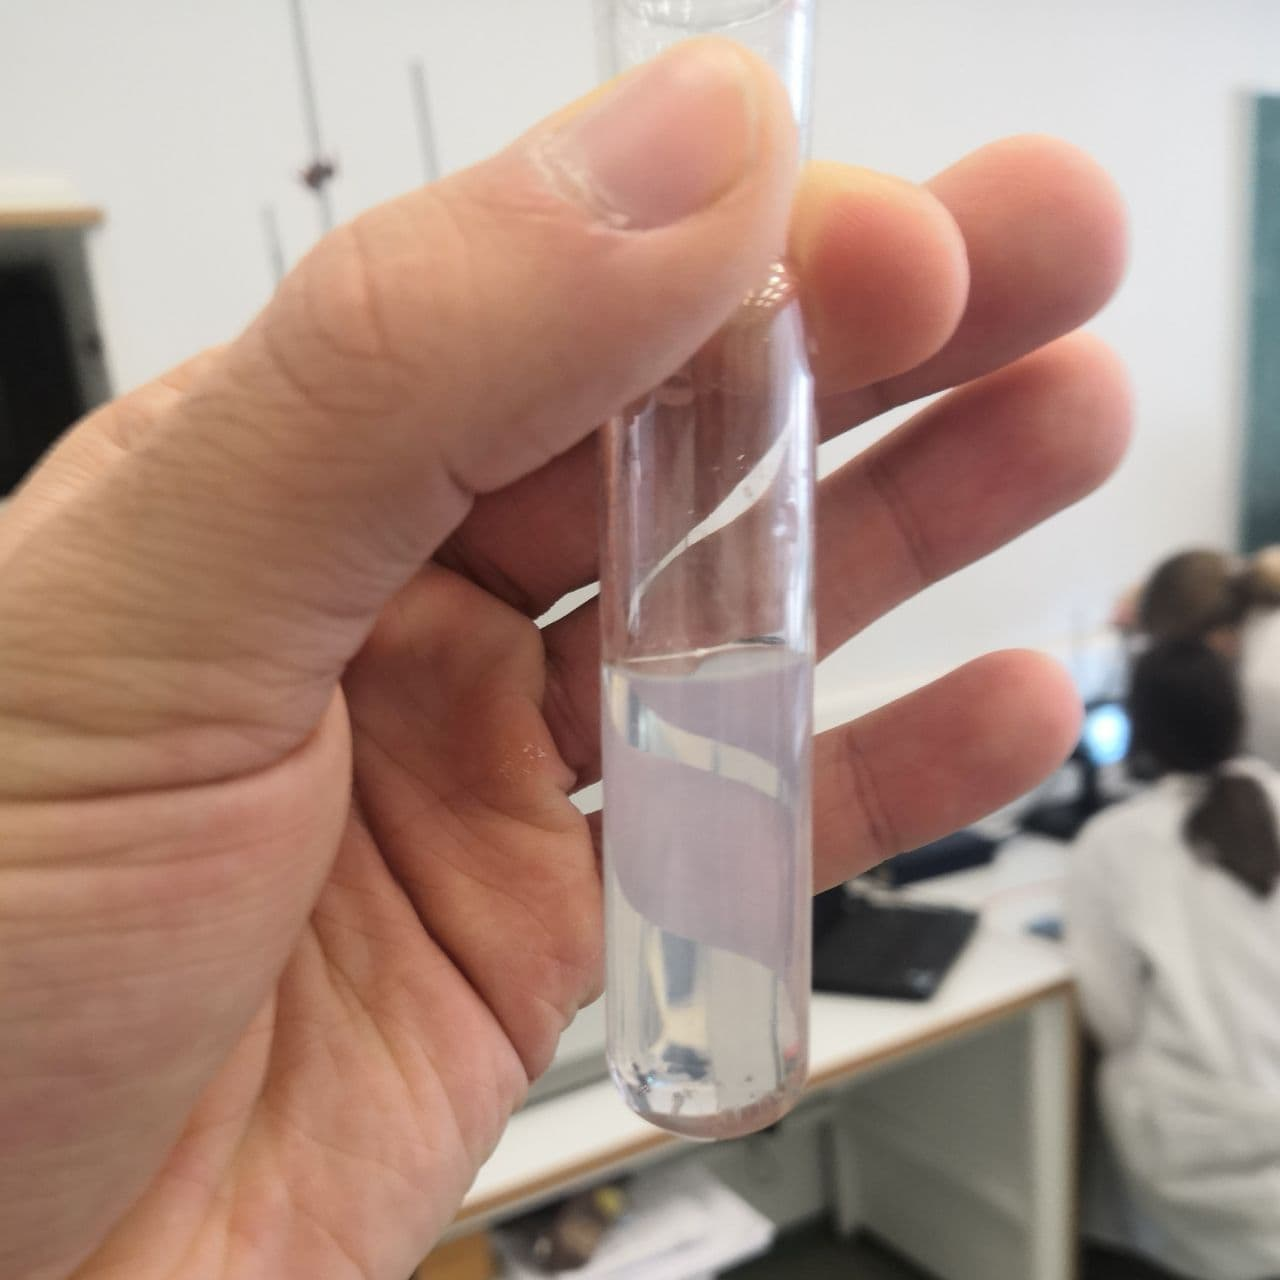
\includegraphics[width=1\linewidth]{photo_2021-03-11_16-32-56.jpg}
\caption{Золь серы, рассеянный свет} %% подпись к рисунку
\label{ris:experimoriginal} %% метка рисунка для ссылки на него
\end{minipage}
\hfill 
\begin{minipage}[h]{0.45\linewidth}
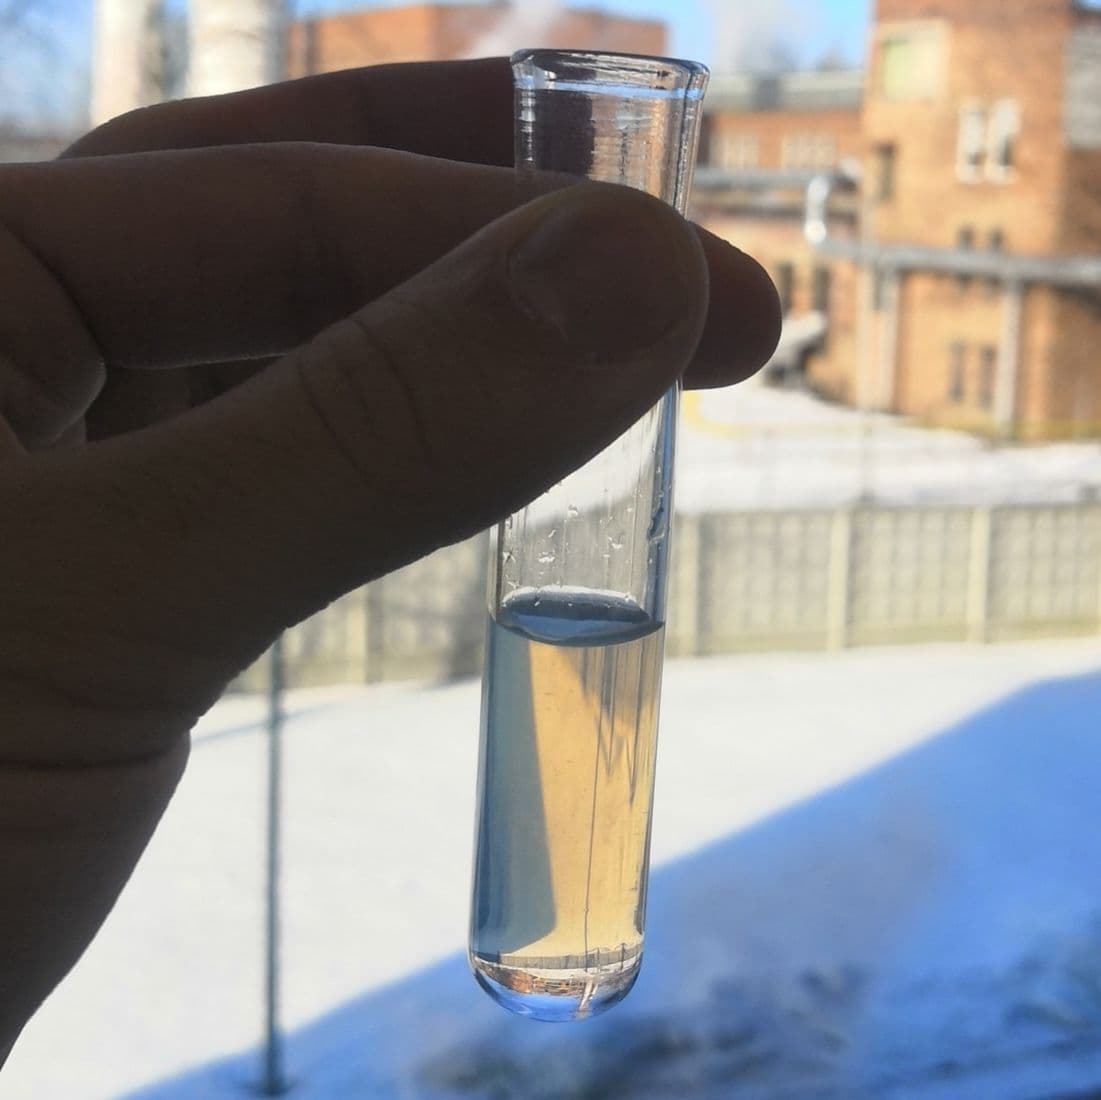
\includegraphics[width=1\linewidth]{photo_2021-03-11_16-33-01.jpg}
\caption{Золь серы, прошедший свет}
\label{ris:experimcoded}
\end{minipage}
\end{center}
\end{figure}

\subsection{Получение золя гидроксида железа $Fe(OH)_{3}$ методом конденсации}
В ~50 мл кипящей воды (в стакане с магнитной мешалкой) добавляется 5 мл 2\%-ного раствора $FeCl_{3}$. 
Гидроксид железа получаемый в результате реакции гидролиза:
$$FeCl_{3} + 3 H_{2}O = Fe(OH)_{3} + 3 HCl$$
стабилизируется ионами железа либо оксохлорида железа (III), образующегося из реакции
$$Fe(OH)_{3} + HCl = FeOCl + 2 H_{2}O.$$
Формула золя:
$$[ [m Fe(OH)3 ] nFeO^{+}(n - x)Cl^{-}]^{x+} xCl^{-} \text{ или } [[m Fe(OH)3 ] nFe^{3+}(3n - x)Cl^{-}]^{x+} xCl^{-}$$
или некоторая их комбинация.

\subsection{Получение золя гидроксида железа $Fe(OH)_{3}$ методом пептизации}
К полупроцетному раствору $FeCl_{3}$ по каплям добавляется 5\%-ный раствор аммиака до тех пор, пока количество
образующегося осадка не перестанет увеличиваться. При этом происходит реакция:
$$FeCl_{3} + 3 NH_{3} H_{2}O = Fe(OH)_{3} + 3NH_{4}Cl.$$
После полного осаждения осадка он декантируется, затем трижды промывается примерно 30мл воды и снова декантируется. Затем осадок взбалтывается в 25мл воды и разливается в 5 пробирок по 2мл в каждую. В каждую пробирку добавляется некоторое количество пептизатора ($FeCl_{3}$), после чего пробирки оставляются на 1 час. В таблице 1 приведены данные о степени пептизации. Обозначения: «-» – отсутствие пептизации, «+, ++, +++» – частичная
пептизация и «++++» - полная пептизация. Фотографии пробирок представлены на рисунке 3.

\begin{table}[h!]
\begin{center}
\caption{Степень пептизации гидроксида железа (III)}
\begin{tabular}{|c|c|c|c|c|c|}
\hline
Пробирка                    & 1 & 2   & 3   & 4   & 5    \\ \hline
Объѐм суспензии Fe(OH)3, мл & 2 & 2   & 2   & 2   & 2    \\ \hline
Объѐм воды, мл              & 5 & 4,8 & 4,6 & 4,4 & 4,2  \\ \hline
Объѐм 10\%-ного FeCl3, мл   & - & 0,2 & 0,4 & 0,6 & 0,8  \\ \hline
Степень пептизации          & - & +   & ++  & +++ & ++++ \\ \hline
\end{tabular}
\end{center}
\end{table}
\begin{figure}[h]
\begin{center}
\begin{minipage}[h]{0.45\linewidth}
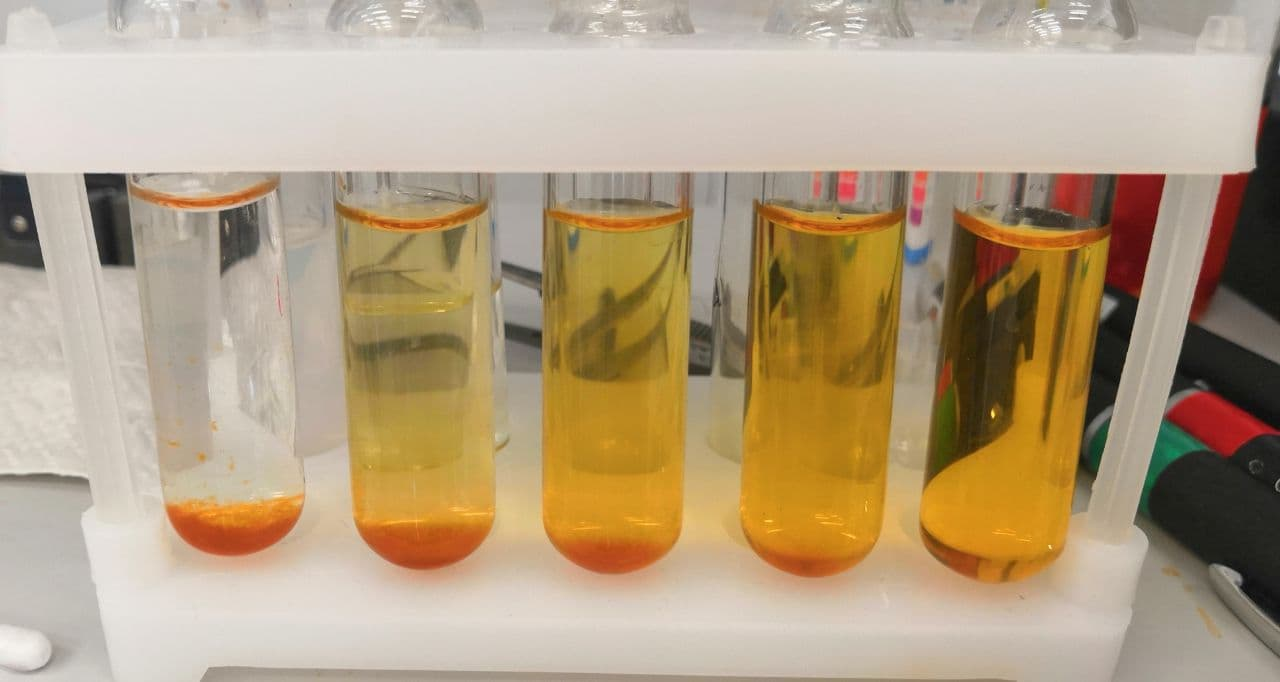
\includegraphics[width=1\textwidth]{photo_2021-03-11_19-04-43.jpg}
\caption{Пробирки с золем гидроксида железа} %% подпись к рисунку
\label{ris:experimoriginal} %% метка рисунка для ссылки на него
\end{minipage}
\hfill 
\begin{minipage}[h]{0.45\linewidth}
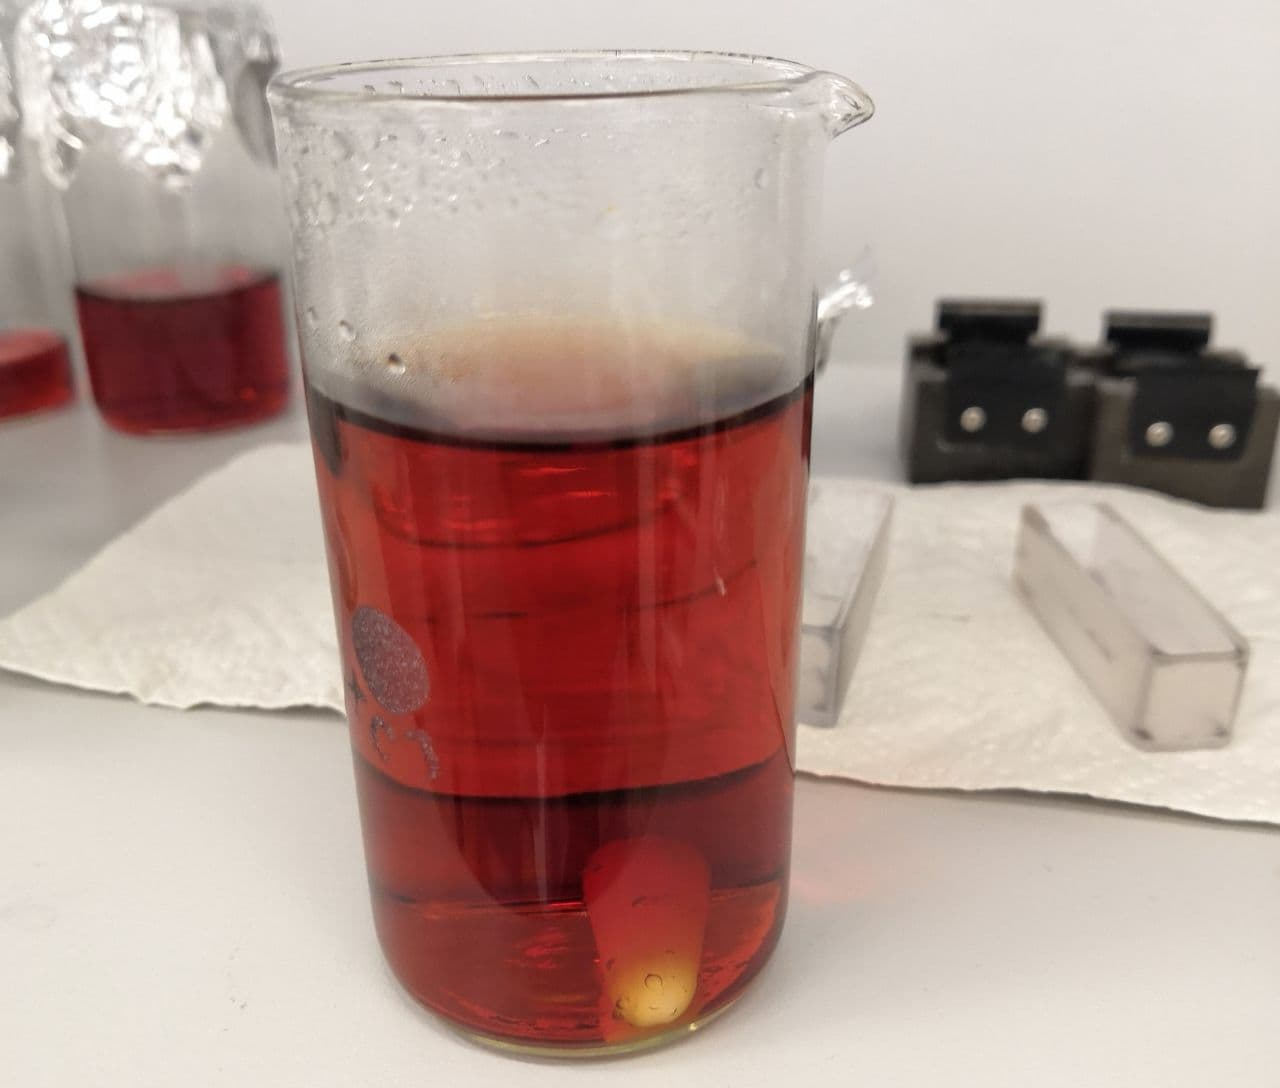
\includegraphics[width=1\textwidth]{photo_2021-03-11_20-30-16.jpg}
\caption{Золь золота}
\label{ris:experimcoded}
\end{minipage}
\end{center}
\end{figure}

Чтобы оценить необходимое количество пептизатора для полного перевода осадка в золь, предположим что весь изначальный хлорид железа прореагировал с аммиаком, мы не потеряли осадок при промывке и равномерно перенесли его во все пробирки тогда отношение необходимого количество пептизатора по отношению к изначальному количеству осадка $x=\frac{n(FeCl_{3})}{n(Fe(OH)_{3})} = (\frac{\frac{2}{25} \cdot 0.5\alpha \cdot \frac{\mu(FeCl_{3})}{\mu(Fe(OH)_{3})}}{0.8\alpha})^{-1}$, где $\alpha$ - коэффициент пересчета объема раствора $FeCl_{3}$ в количество вещества. Итого, в такой грубой оценке $x \simeq 13 $, что говорит о том что количество пептизатора в растворе должно превышать количество осадка минимум на порядок.

\subsection{Получение золя золота}
В 50 мл дистиллированной воды, нагретой до кипения, добавляется 0.5 мл 1\% раствора $HAuCl_{4}$, и потом послу трёх минут кипячения при размешивании добавляется 0.9 мл раствора $Na_{3}Cyt$. Раствор кипятится несколько минут до тех пор, пока окраска не перестанет меняться. Затем золь охлаждается до 40 градусов и хранится для следующих экспериментов (рис. 4). 
Реакция цитратного восстановления:
$$2HAuCl_{4} + 3Na_{3}Cyt\rightarrow 2Au+3Na_{2}O=C-(CH_{2}COO)_{2}+3CO_{2}+3NaCl+5HCl.$$
Формула золя:
$$[ [m Au ] nCyt^{3-}(3n - x)Na^{+}]^{x-} xNa^{+}$$
Молярные массы: $\mu(Na_{3}Cyt)$ = 258 г/моль, $\mu(HAuCl_{4})$ = 340 г/моль. Значит, был добавлен избыток цитрата натрия и можно считать, что все золото в растворе находиться в коллоидной форме. Оценим объемную концентрацию мицелл.
\begin{figure}[h]
\begin{center}
\begin{minipage}[h]{0.49\linewidth}
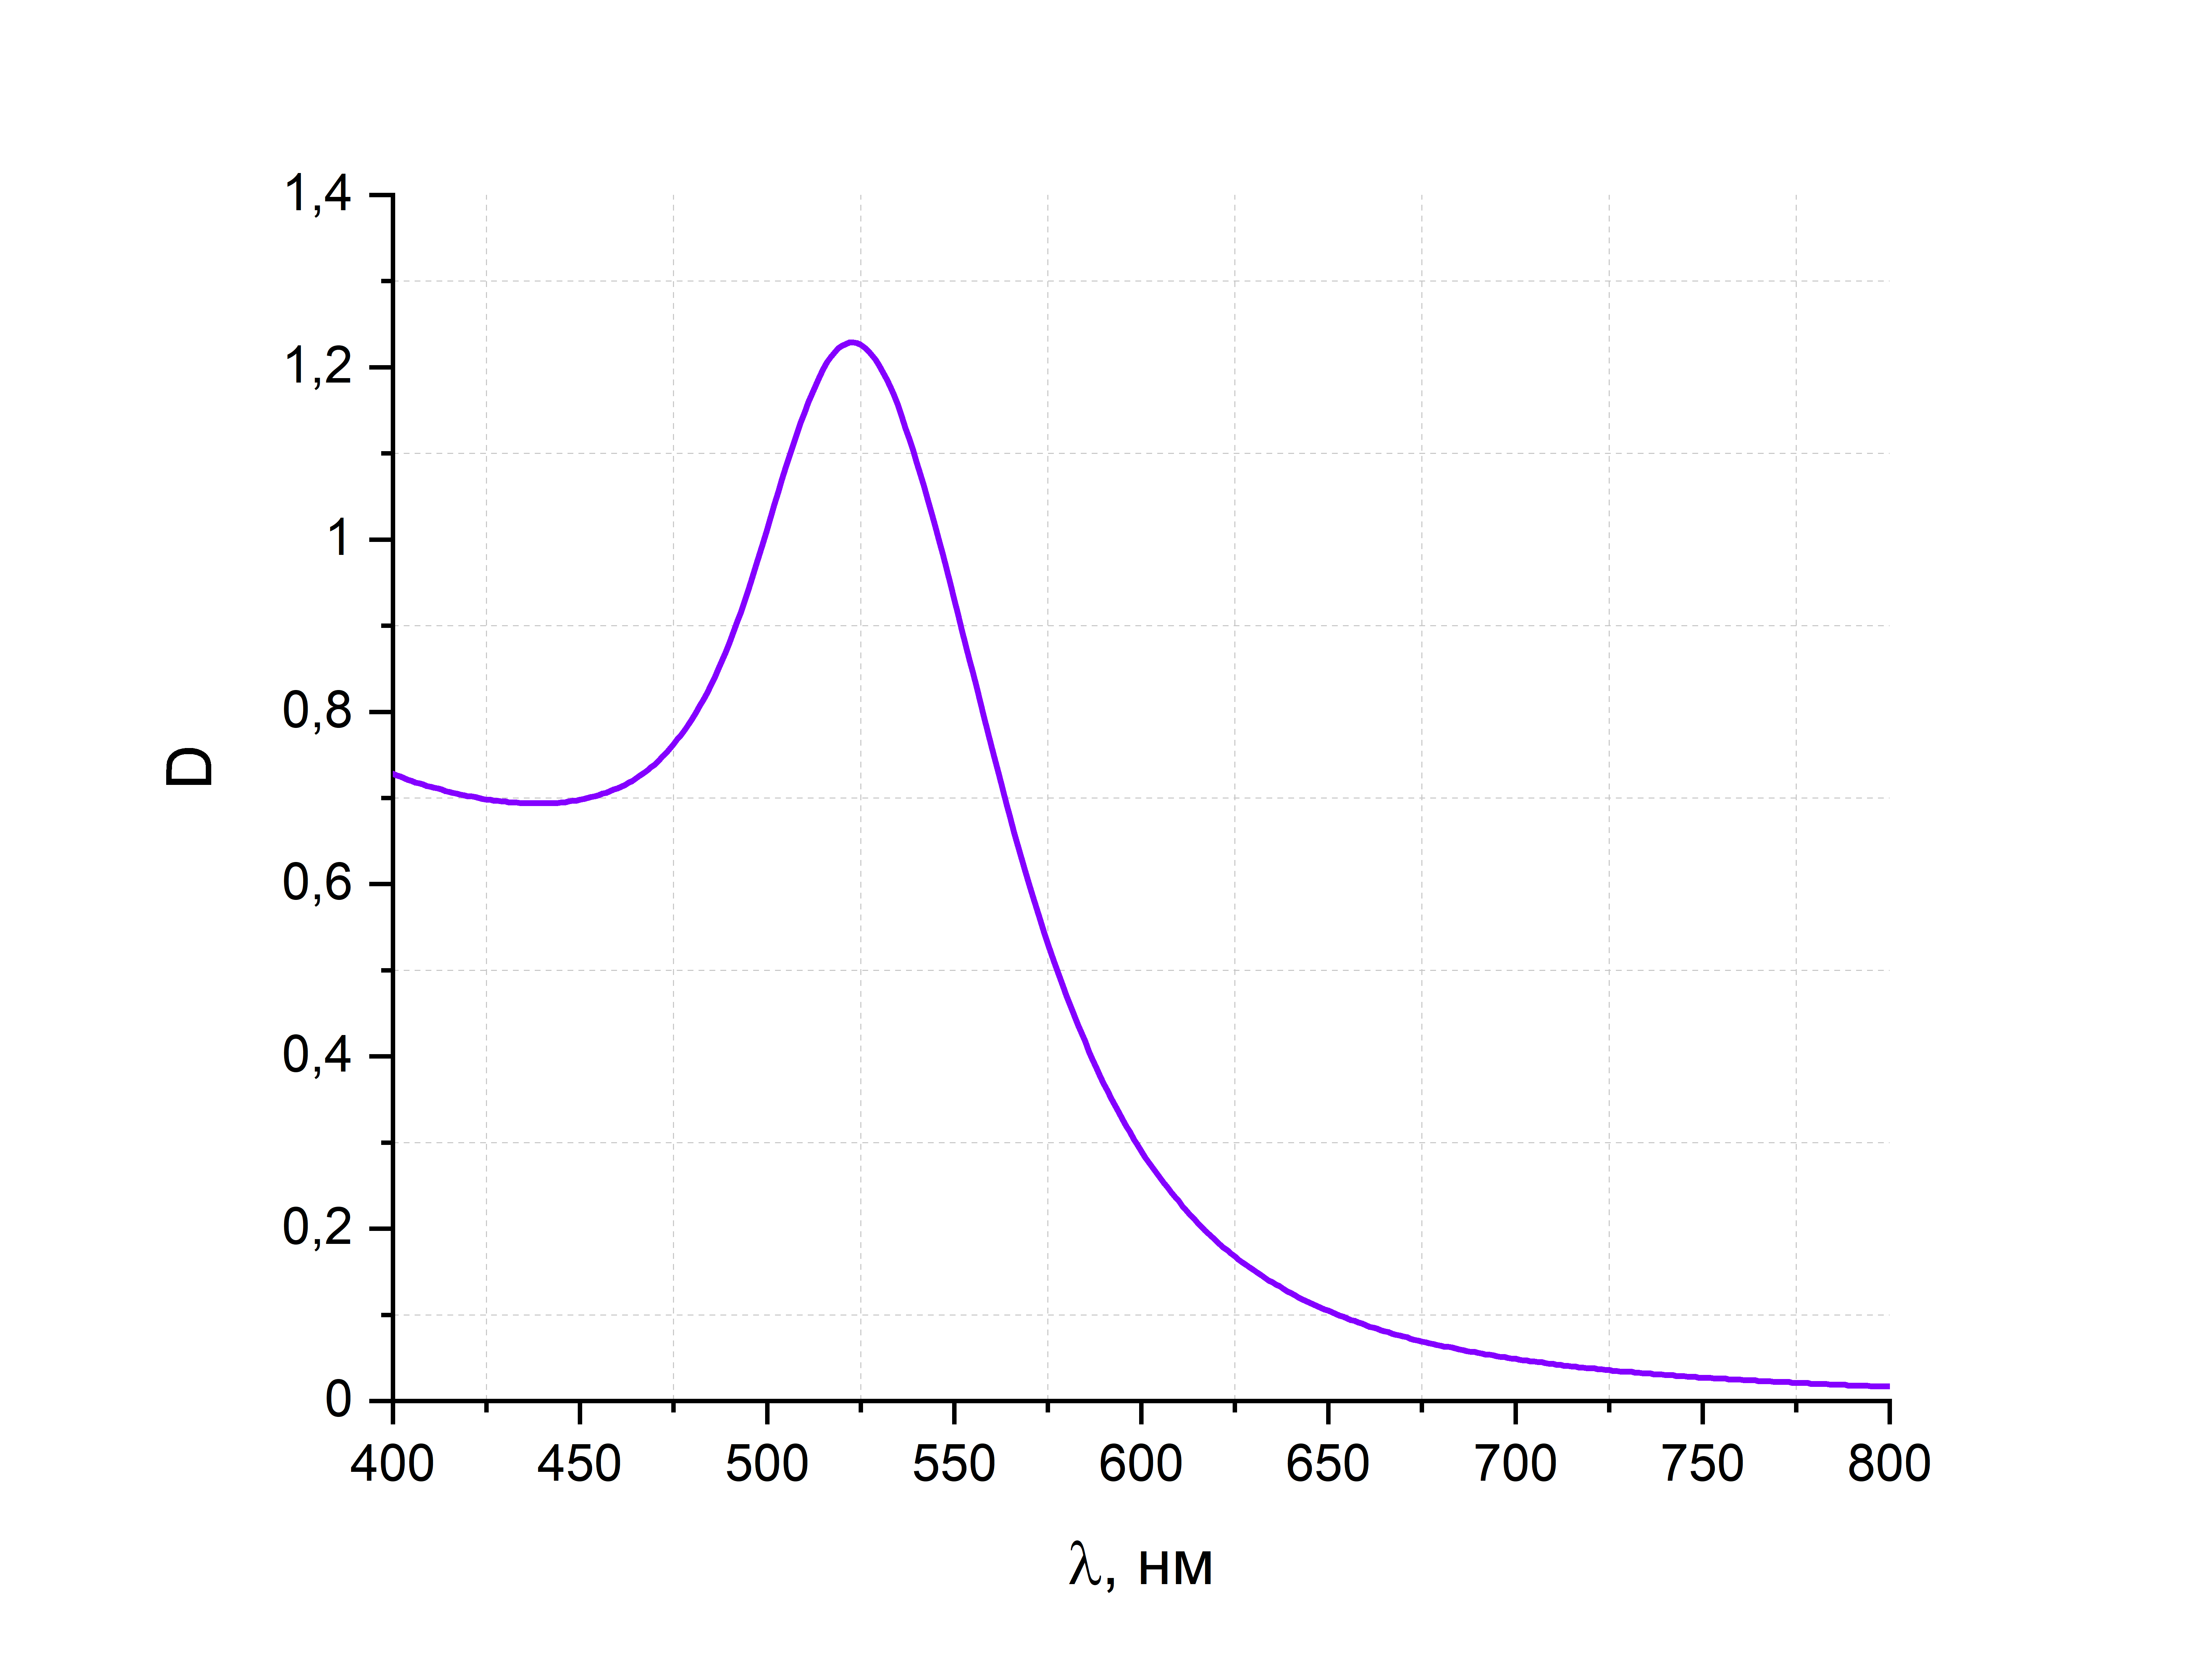
\includegraphics[width=1\textwidth]{abs.png}
\caption{Спектр поглощения золя золота} %% подпись к рисунку
\label{ris:experimoriginal} %% метка рисунка для ссылки на него
\end{minipage}
\hfill 
\begin{minipage}[h]{0.49\linewidth}
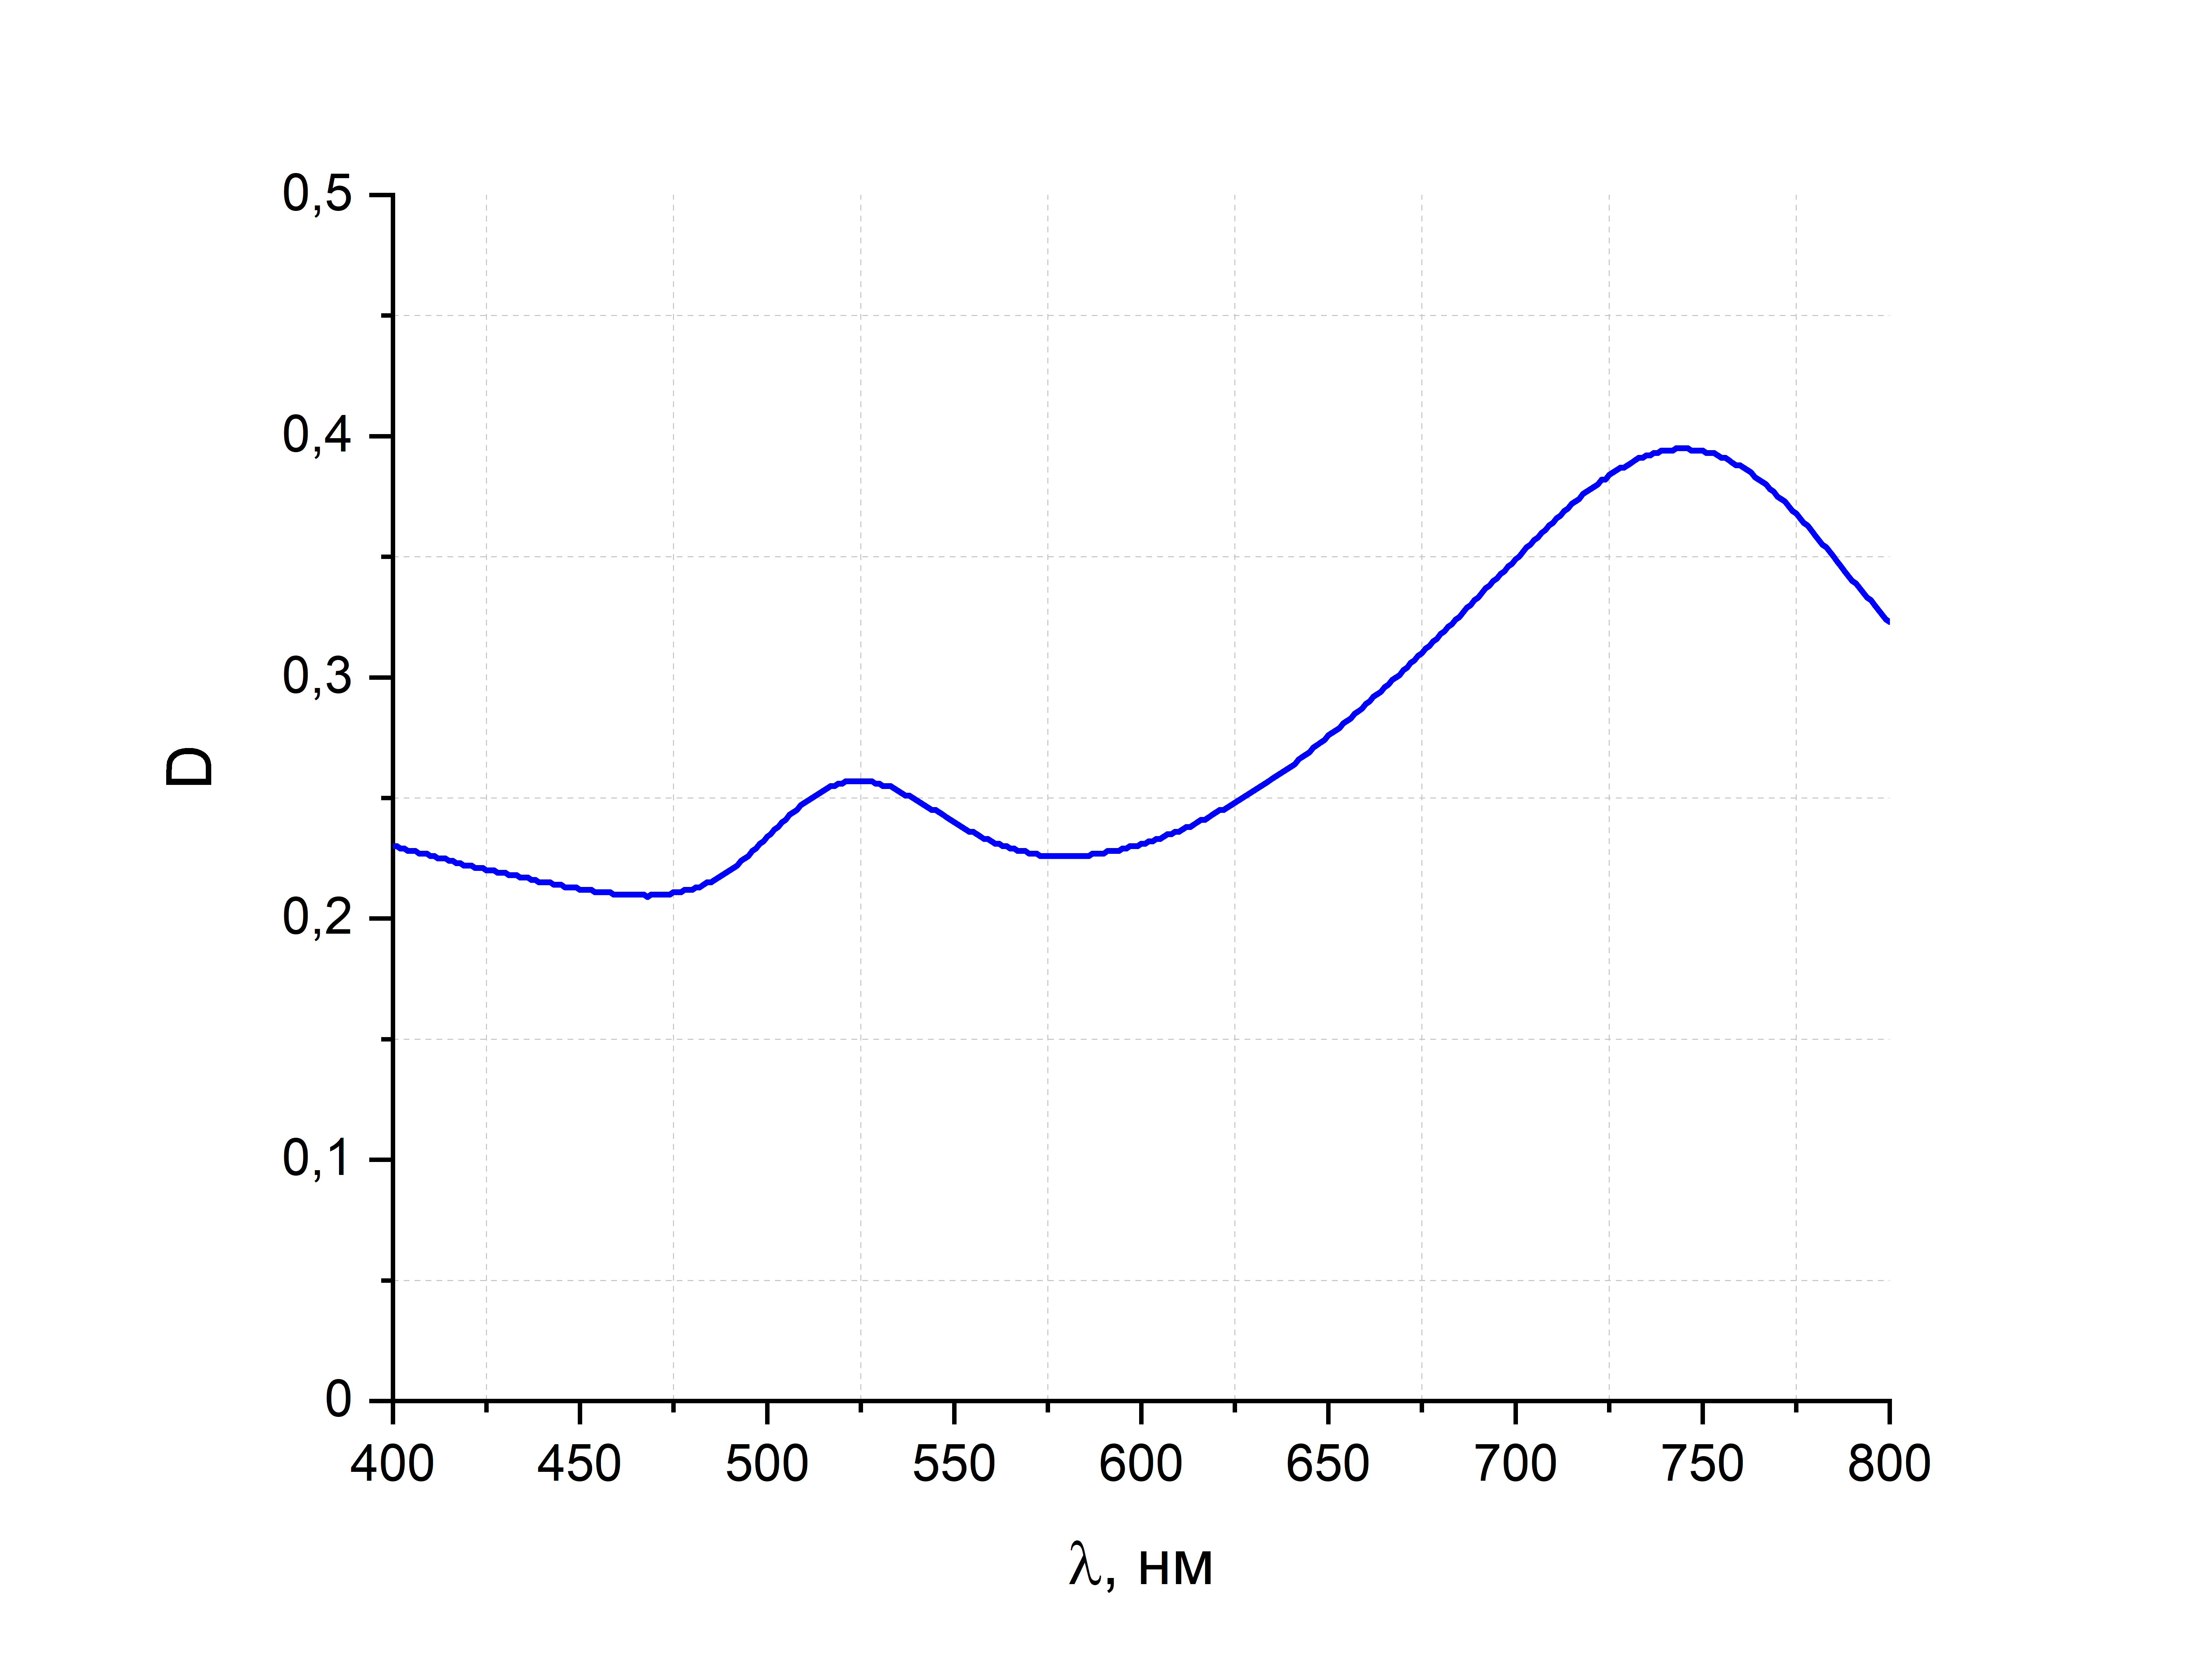
\includegraphics[width=1\textwidth]{abs_coag.png}
\caption{Спектр скоагулировавшего золя}
\label{ris:experimcoded}
\end{minipage}
\end{center}
\end{figure}

Для этого снимается спектр поглощения золя (рис. 5) и через максимум поглощения рассчитывается\footnote{J. Phys. Chem. C2007,111,14664-1466} размер частиц:
$$
\lambda_{\max }=518.8-0.0172 d+0.0063 d^{2}-0.0000134 d^{3}=522\div523\text{ нм} => d = 26.4 \pm 1.7\text{ нм}
$$
Тогда количество частиц золота, приходящихся на одну мицеллу:
$$
\alpha = \frac{\rho_{Au}\frac{\pi d^3}{6}}{\mu(Au)} N_{a}= 570  000 \pm 120 000
$$
Таким образом, полное число частиц золя в растворе:
$$
N_{nAu} = \frac{N_{HAuCl_{4}}}{\alpha}=\frac{N_{a}m_{HauCl_{4}}\cdot1\%}{\alpha\mu(HAuCl_{4})} = (1.6 \pm 0.3)\cdot 10^{13}, \text{ }
C_{nAu} = \frac{N_{nAu}}{N_{a}V} = (4.5 \pm 0.9)\cdot10^{-10} M
$$



\subsection{Определение порогов коагуляции золя золота}
Для определения порогов электролитной коагуляции берутся растворы солей с разными зарядами противоиона. (+1, +2, +3) В кювету вводят по 2 мл электролитов разной концентрации и 1 мл исследуемого золя. По времени изменения цвета раствора определяется, является ли коагуляция быстрой (Из теории коагуляции Смолуховского: $\tau_{1/2} \simeq 0.6c$). Брались соли: $KNO_{3}$(0.5M), $Mg(NO_{3})_{2}$(0.01M), $La(NO_{3})_{3}$(0.001M) Результаты в Таблице 2.

\begin{table}[h!]
\begin{center}
\caption{Измерение С_{\text{пк}}}
\begin{tabular}{|c|c|c|c|c|c|}
\hline
$V_{KNO_{3}}$, мкл & Коагуляция  &$V_{Mg(NO_{3})_{2}}$, мкл               & Коагуляция            & $V_{La(NO_{3})_{3}}$, мкл               & Коаугляция            \\ \hline
2000          & б           & 300                   & м                     & 500                   & м                     \\ \hline
1000          & б           & 350                   & б                     & 750                   & б                     \\ \hline
500           & б           & 400                   & б                     & 625                   & м                     \\ \hline
250           & м           & 550                   & м                     & 680                   & б                     \\ \hline
375           & б           & \multicolumn{1}{l|}{} & \multicolumn{1}{l|}{} & 650                   & м                     \\ \hline
310           & б           & \multicolumn{1}{l|}{} & \multicolumn{1}{l|}{} & \multicolumn{1}{l|}{} & \multicolumn{1}{l|}{} \\ \hline
280           & б($\sim$1с) & \multicolumn{1}{l|}{} & \multicolumn{1}{l|}{} & \multicolumn{1}{l|}{} & \multicolumn{1}{l|}{} \\ \hline
\end{tabular}
\end{center}
\end{table}

\begin{table}[h!]
\begin{center}
\caption{Пороги коагуляции}
\begin{tabular}{|l|l|l|ll}
\cline{1-3}
z & V_{\text{соль}}, мкл  & С_{\text{пк}}, мМ &  &  \\ \cline{1-3}
1 & 280 \pm 30  & 47 \pm 5     &  &  \\ \cline{1-3}
2 & 350 \pm 50  & 1.17 \pm 0.17  &  &  \\ \cline{1-3}
3 & 680 \pm 30  & 0.2267 \pm 0.0010 &  &  \\ \cline{1-3}
\end{tabular} 
\end{center}
\end{table}

Т.о соотношение порогов коагуляции исследованных электролитов для трёх-, двух-, и однозарядных ионов: 1:5:206. Согласно правилам Дерягина-Ландау и Эйлерса-Корфа: $C_{\text{пк}} \sim \frac{1}{z^n}$ (n=6 и n=2 соотв.) Построим график зависимости $C_{\text{пк}}$ от заряда противоиона в двойных логарифмических координатах для нахождения порядка n. См.Рис.7



\begin{figure}[h]
\begin{center}
\begin{minipage}[h]{0.45\linewidth}
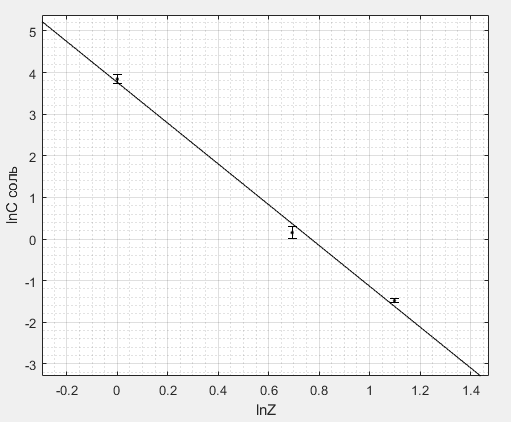
\includegraphics[width=1\textwidth]{2.1_lnC(lnZ).png}
\caption{График зависимости lnC(lnZ)} %% подпись к рисунку
\label{ris:experimoriginal} %% метка рисунка для ссылки на него
\end{minipage}
\hfill 
\begin{minipage}[h]{0.5\linewidth}
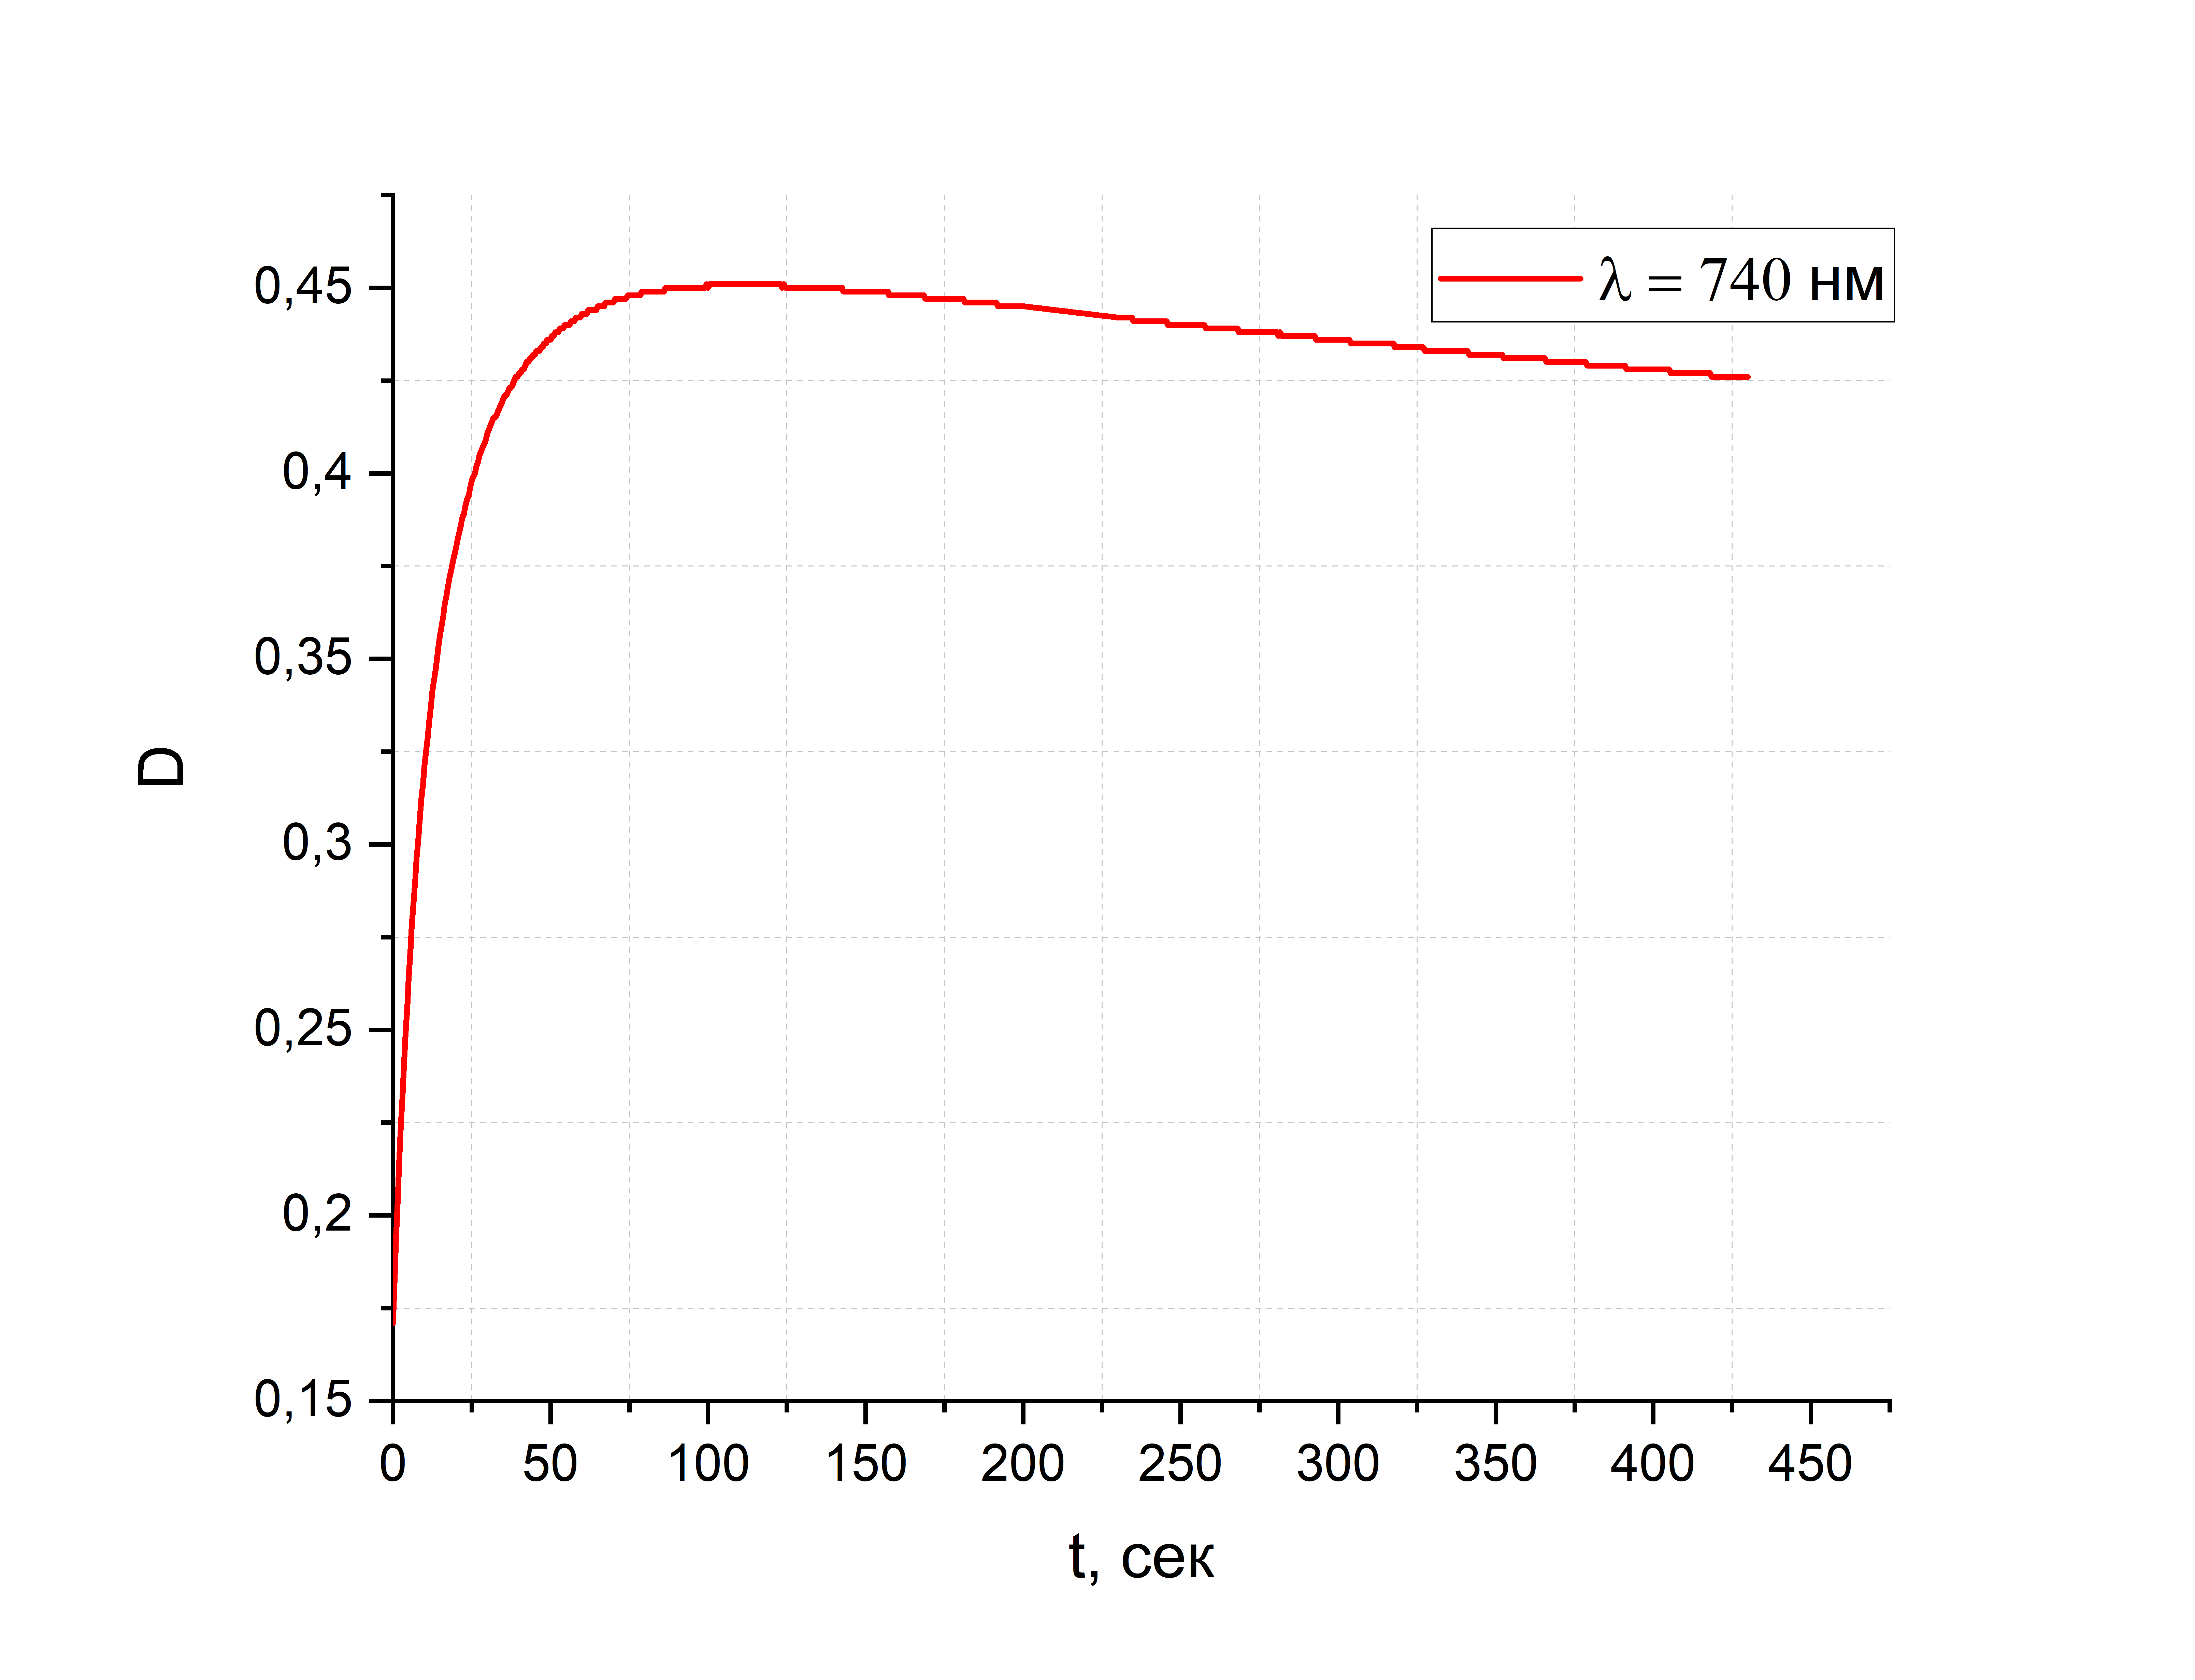
\includegraphics[width=1\textwidth]{time_coag.png}
\caption{D(t) для медленной коагуляции}
\label{ris:experimcoded}
\end{minipage}
\end{center}
\end{figure}


Получили $n = 4.9 \pm 0.3$. 

Для одной из солей концентрации, близкой к пороговой (0.217mM $La(NO_{3})_{3}$), пронаблюдали временную зависимость показателя оптической плотности раствора от времени (на длине волны $\lambda = 740nm$ , т.к это - пик поглощения у коагулировавшего раствора). Результаты на Рис.8  
\newpage
%%%%%%%%%%%%%%%%%%%%%%%%%%%%%%%%%%%%%%%%%%%%%%%%%%%%%%%%%%%%%%%%%%%%%%%%%
 \section{Выводы}
\begin{enumerate}
    \item Были приготовлены золь серы методом замены растворителя, золи гидроксида железа (III) методами конденсации и пептизации. На полученных золях можно было пронаблюдать такие характерные явления как опалесценция и конус Тиндаля (см рис. 9, 10).
    \item Получен отрицательный золь золота с размером частиц $d = 26.4\pm1.7$нм. Концентрация частиц золя $(3.0\pm 0.6)\cdot 10^{17} \text{м}^{-3}$.
    \item Определены пороги коагуляции для солей с разными зарядами противоионов. Найдена степень зависимости $C_{\text{пк}} \sim z^{-n}$, $n=4.9 \pm 0.3$. Откуда можно сделать вывод, что имеют место оба механизма электролитной коагуляции, но концентрационная в большей мере. (4.9 ближе к 6, чем к 2)

\end{enumerate}

\begin{figure}[h]
\begin{center}
\begin{minipage}[h]{0.44\linewidth}
\begin{center}
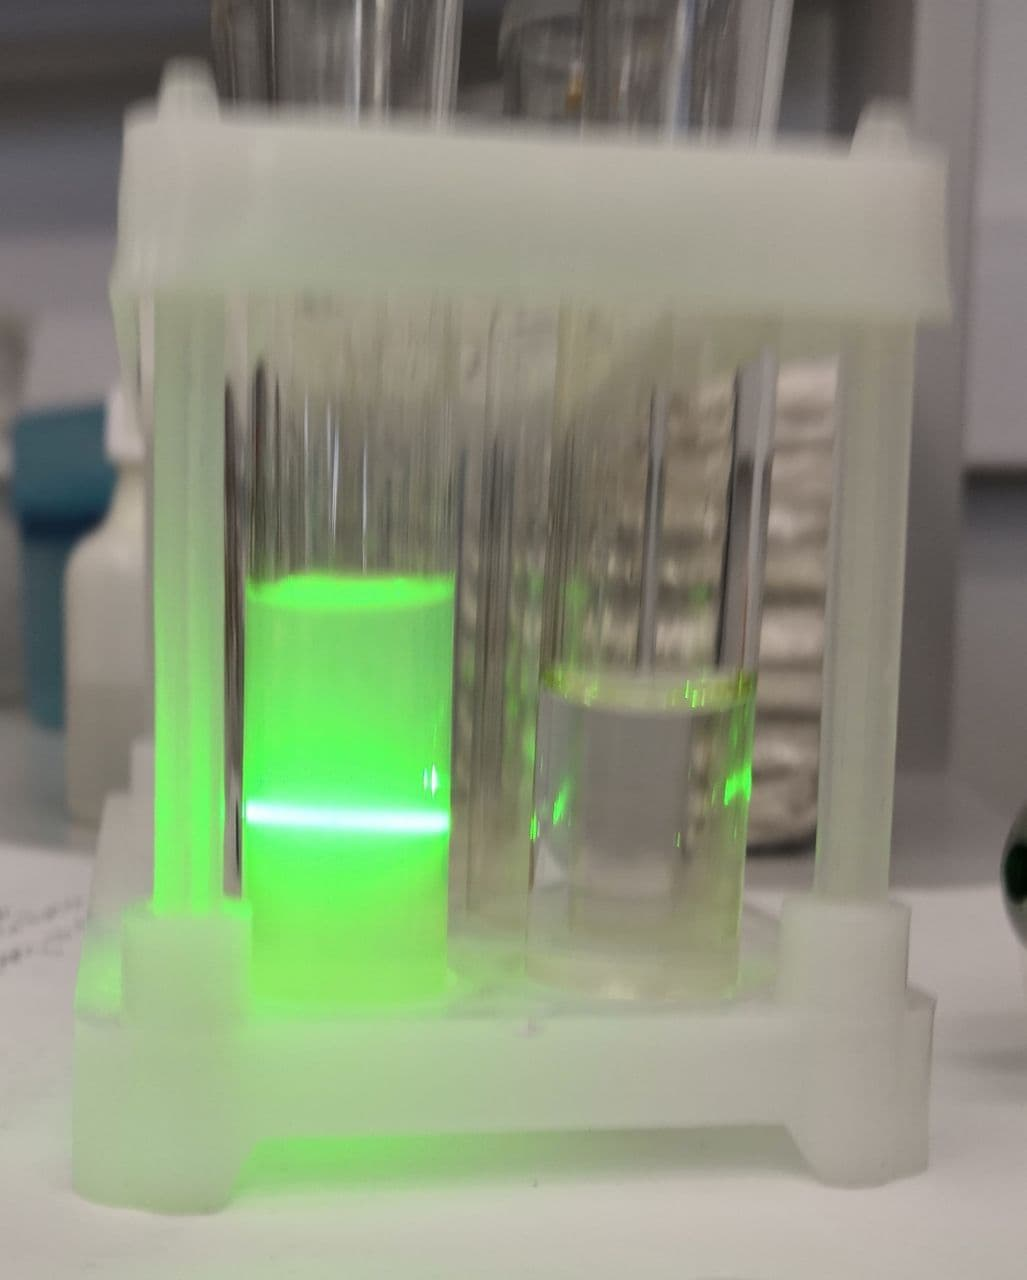
\includegraphics[width=0.6\textwidth]{photo_2021-03-12_18-41-31.jpg}
\caption{Просвет лазером золя S} %% подпись к рисунку
\label{ris:experimoriginal} %% метка рисунка для ссылки на него
\end{center}
\end{minipage}
\hfill 
\begin{minipage}[h]{0.44\linewidth}
\begin{center}
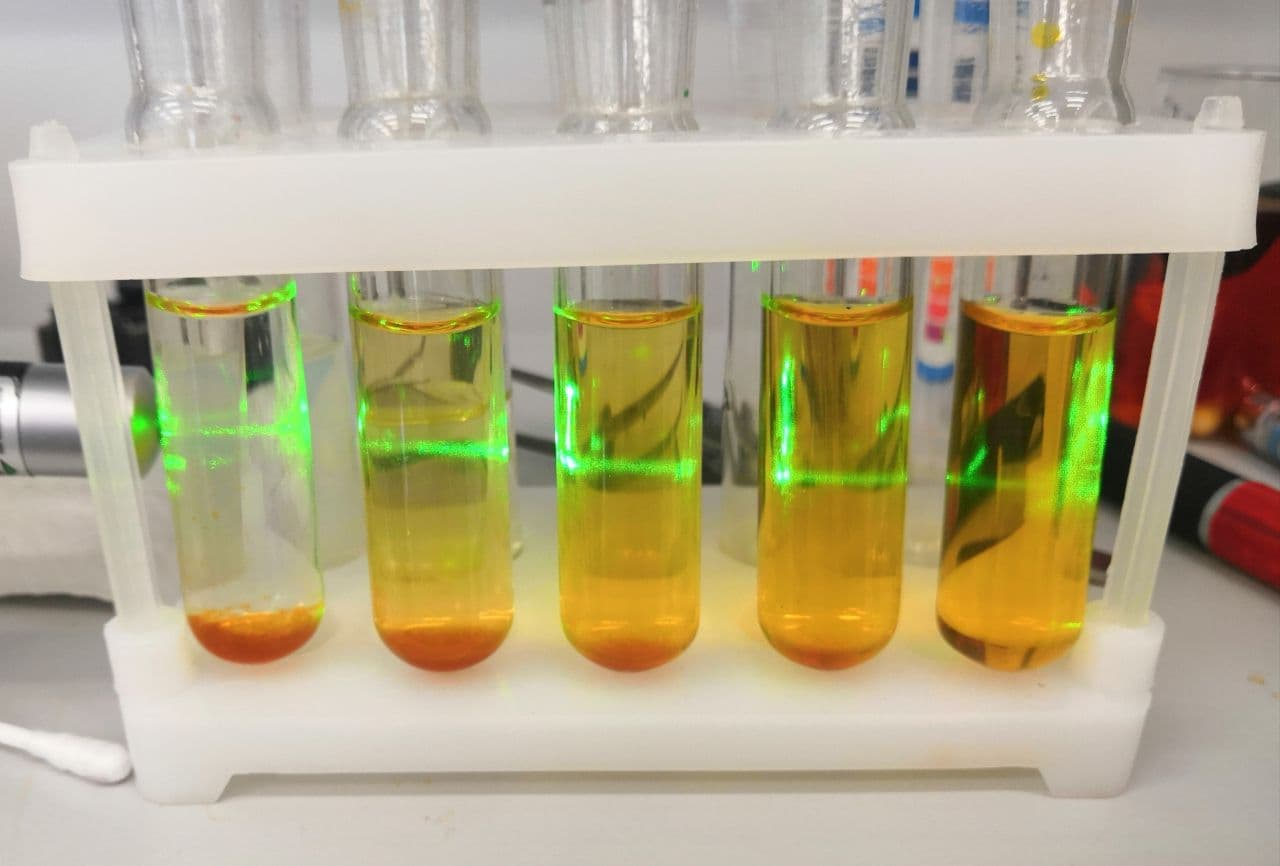
\includegraphics[width=1\textwidth]{photo_2021-03-12_18-41-28.jpg}
\caption{Просвет лазером золя гидроксида железа}
\label{ris:experimcoded}
\end{center}
\end{minipage}
\end{center}
\end{figure}
%%%%%%%%%%%%%%%%%%%%%%%%%%%%%%%%%%%%%%%%%%%%%%%%%%%%%%%%%%%%%%%%%%%%%%%%%
% \section{Приложения}


\end{document}
\begin{figure}[h!]
    \begin{center}
    \includegraphics[width=0.8\textwidth]{xxx.png}
    \end{center}
    \caption{...}
\end{figure}
